\documentclass[conference]{IEEEtran}
\IEEEoverridecommandlockouts
% The preceding line is only needed to identify funding in the first footnote. If that is unneeded, please comment it out.
\usepackage{cite}
\usepackage{amsmath,amssymb,amsfonts}
\usepackage{algorithmic}
\usepackage{graphicx}
\usepackage{textcomp}
\usepackage{xcolor}
\def\BibTeX{{\rm B\kern-.05em{\sc i\kern-.025em b}\kern-.08em
    T\kern-.1667em\lower.7ex\hbox{E}\kern-.125emX}}
\begin{document}


\title{Sentiment Analysis of Twitter Covid-19 Vaccine Dataset using Deep Learning Techniques}

\author{\IEEEauthorblockN{Dorodi Afroze Krishty}
\IEEEauthorblockA{\textit{Dept. of Systems Design Engineering} \\
\textit{University of Waterloo}\\
Waterloo, Canada \\
dkrishty@uwaterloo.ca}

}

\maketitle

\begin{abstract}

Sentiment analysis deals with identifying and classifying opinions or sentiments expressed in source text. Sentiment analysis of this user generated data is very useful in knowing the opinion of the crowd. The objective of this work is to automate the process of sentiment analysis by applying deep neural network for predicting three different sentiments (positive, neutral, negative) on twitter Covid-19 vaccine dataset. The classifier model will be trained on a pre-existing labelled twitter dataset for general purpose use and then by utilising transfer learning method the trained model will be repurposed on the Covid-19 vaccine dataset to generate labels or sentiments based on the text data. 
\end{abstract}

\begin{IEEEkeywords}
% 2-5 keywords don't use generics ones like Machine-Learning (be more specific)
Twitter, NLP, Sentiment Analysis, Long Short Term Memory Recurrent Neural Network, Convolutional Neural Network, Transfer Learning
\end{IEEEkeywords}


% Sections
\section{Introduction} \label{sec:intro}
The first Covid-19 case was identified in December 2019 and has now spread evidently all across the world. As of July 31st, the World Health Organisation (WHO) confirms over 196 million cases and over 4 million resulting in deaths worldwide~\cite{dworld}. For over more than a year now, the economic and social disruption caused by the pandemic is devastating and lives have not been the same.

Over the past year, many vaccines have been developed and approved with Oxford-Astrazanica, Pfizer BioNtech, Sinopharm, and Moderna being the most popular ones as per the New York Times (NYT)~\cite{fworld}. Around 28.8\% of the world population has received at least 1st dose of a Covid-19 vaccine and over 14 percent is fully vaccinated and most of this population resides in high-income countries~\cite{eworld}. 

Even though all the approved vaccines underwent rigorous safety checks and protocols before approval, certain people are skeptical and fearful concerning the safety of vaccines. For vaccinations to be successful in fighting off Covid-19 successfully, it is of utmost necessity to understand and identify the fear and misconceptions in the general community so they can be dealt with accordingly. Every day, humans interact through public social media exchanging large quantities of freely available data with each other.  This data is extremely valuable in understanding human behavior. Therefore, social media platforms like Twitter are a comprehensive source of data needed to understand the public sentiment on vaccines. By performing Natural Language Processing (NLP) using deep learning techniques on a data set to classify tweets can provide a general public sentiment towards vaccines. This will help in achieving a comprehensive interpretation of the data which can be used to identify potential misconceptions and fears. These issues can then be addressed accordingly and help increase vaccination rates.

To fulfil the objective of Sentiment Analysis on Twitter Covid-19 Vaccine data, we conduct extensive experiments over two datasets and leverage the widely-used convolutional neural network (CNN) and long short term memory (LSTM)-based recurrent neural network (RNN) as
our models. And we try to systematically transfer neural network by learning the features from a sentence level Sentiment Analysis approach. 
\\


\section{Background}\label{sec:background}

%%%%%%%%%%%%%%%%%%%%%%%%%%%%%%

Natural Language Processing (NLP) combines the field of linguistics and computer science to decipher a language structure and guidelines to make models which can comprehend, break down and separate significant details from text or speech. Sentiment Analysis is a technique in NLP, which identifies and categorizes opinions from a piece of text that determines the emotional as well as attitude of the writer towards a particular topic \cite{feldman2013techniques}. There are three main classification levels namely: document level, sentence level and aspect level. Both document and sentence level sentiment analysis aims to classify the negative or positive opinion or sentiment. In the aspect level the Sentiment Analysis technique aims to classify the sentiment with respect to the specific aspects of entities. \cite{medhat2014sentiment}. \\
Another crucial aspect of NLP applications is word representations. It is common to represent words as indices in a vocabulary, but this fails to capture the rich relational structure of the lexicon. Vector-based models do much better in this regard. They encode continuous similarities between words as distance or angle between word vectors in a high-dimensional space \cite{ maas2011learning}. One of the first breakthrough architecture in word representations that came out was Embedding from Language Models (Elmo) because it created embeddings that preserved context. It contained two bidirectional RNNs trained for language modelling. Authon in ~\cite{peters2018deep} proposed a general approach for learning high-quality deep context-dependent representations from biLMs and showed large improvements when applying Elmo to an extensive range of NLP tasks.\\
Recently, deep learning has become a popular approach for Sentiment Analysis task in NLP applications and many studies have been devoted to build powerful feature extraction tools.

Deep learning includes many networks such as CNN (Convolutional Neural Networks), RNN (Recurrent Neural Networks), Recursive Neural Networks, DBN (Deep Belief Networks) and many more. Neural networks are very beneficial in text generation, vector representation, word representation estimation, sentence classification, sentence modeling and feature presentation \cite{ zhang2016sentiment}.  

Lately, a variety of model designs and methods have been worked on in the context of NLP. 
In a study by \cite{ li2014identifying} a modification of RNN called Recursive Tensor Network (RTN) was was for sentiment analysis on online review corpus, the proposed model was compared with Naïve Bayes, KNN and SVM based models. The effectiveness of the deep learning model showed superior outcomes than the shallow classifiers. 
A study by \cite{ ouyang2015sentiment} presented a seven-layer CNN and Word2Vec (proposed by Google) for Sentiment Analysis on movie reviews’ excerpt. By comparing the proposed model with previous models such as Matrix-Vector recursive neural network (MV-RNN) and recursive neural network (RNN), the proposed model outperformed the previous models with 45.5 \% accuracy. 

The authors in~\cite{zhou2015c}  combined  a CNN to extract a sequence of higher-level phrase representations that are fed into an LSTM to obtain the sentence representation. Their model captured both local features of phrases as well as global and temporal sentence semantics. Their results showed that their model by using both CNN and LSTM can achieve exceptional performance on Sentiment Analysis tasks.



Twitter is an important microblogging domain as such Twitter based Sentiment Analysis has shown to help analyse critical information regarding Covid-19 pandemic and people’s reaction towards Covid-19 vaccines. Several papers have demonstrated interesting techniques from traditional machine learning approach to deep neural networks. Sentiment Analysis of Twitter phrases has proven to be a rather challenging task but has also led to developments in the algorithms and techniques that are utilised. For instance, authors in \cite{na2021insight} collected tweet posts by the UK and US users using the Twitter API during the pandemic and designed experiments to answer some pressing questions concerning vaccination. They performed sentiment analysis by using the pretrained model VADER~\cite{hutto2014vader} and proposed a new method that can count the individual’s influence. Pre-trained models like the VADER can learn the basics of a language and become useful on a host of other NLP tasks via transfer learning. \\
In fact, in Sentiment Analysis, transfer learning method can be applied to transfer sentiment classification from one domain to another \cite{tan2011weighted}. It is particularly important to neural networks, which are very likely to be overfitting \cite{mou2016transferable}. It has proven efficient in image processing, but conclusions are still being tested regarding NLP applications. Previous neural NLP studies have casually applied transfer techniques, but their results are not consistent. Therefore, more systematic studies are needed to shed light on transferring neural networks in the field of NLP.


%%%%%%%%%%%%%%%%%%%%%%%%%%%%%%%


\section{Method} \label{sec:method}

The methodology is based on 5 important aspects that represents our NLP workflow and focuses on a strategy for sentiment analysis on Twitter data. The architectural overview describing the overall process of sentiment analysis is shown in Figure~\ref{fig:fig1}

\textbf{Training Data:} The training dataset called 'Sentiment Extraction Twitter Dataset'~\cite{bworld} consists of 27,400 words or phrases fetched from twitter and labelled with the corresponding sentiment (positive, negative and neutral). Upon initial exploratory data analysis the dataset was found to have a distribution of 40\% neutral, 31\% positive and 28\% negative data. This particular dataset involves general tweets from the public and is not focused on any particular topic.

\textbf{Preprocessing:} In its raw form, text data or tweets add no meaningful information for machine learning predictions. To uncover the sentiment behind a tweet, the raw text data was cleaned using Natural Language Toolkit (NLTK). This consisted of tokenization, stemmming, lemmatization, stopwords removal, parts of speech tagging, URL removal, word embeddings, followed by encoding the labels.

Embedding layer is an essential part of neural network as we will see.  As such, representing words using a dense vector helps improve model over sparse representation such as simpler Bag of Words (BoW) representation. We use a Keras word embedding layer to fit our neural network on text. The Embedding has a vocabulary of 5000 words and a dimension of 200. Embeddings are a great way to deal with NLP problems as they help with dimensionality reduction over one hot-encoding as we can control the number of features.\

\textbf{Classifier Model:} Based on the classifier model, the system evaluates whether the tweet is positive, negative or neutral. We will employ deep neural networks such as LSTM and CNN to evaluate the best performing model based on the supervised feature learning on the training dataset. 

\textbf{Covid-19 vaccine dataset:} The Covid-19 vaccine dataset does not contain labelled data, so an additional training dataset was initially used to train the classifier model, which has learned features from the training dataset to evaluate the sentiments of the Twitter Covid-19 Vaccines Dataset ~\cite{cworld}.This dataset consists of recent tweets about the Covid-19 vaccines from all across the world namely: 
\begin{itemize}
    \item Pfizer/BioNTech
    \item Sinopharm
    \item Sinovac
    \item Moderna 
    \item Oxford/AstraZeneca
    \item Covaxin 
    \item Sputnik V
\end{itemize}

\textbf{Transfer Learning:} Many  machine  learning  techniques  rely  on  the  availability of  labelled  training  data.  Ideally,  this  training  data  should be  available  in  abundance  to  simplify  the  training  procedure and  improve  the  performance  of  the  trained  models. In the domain of sentiment analysis, annotating texts like tweets is an arduous task because of the high frequency of new tweets everyday. Transfer Learning presents the opportunity for deep learning models to be re-purposed for another task. As such, by training a neural network on the annotated 'Sentiment Extraction Twitter Dataset' it is possible to fit the analysis of our 'Twitter Covid-19 Vaccine Dataset'. 


\begin{figure}[h]
\centering
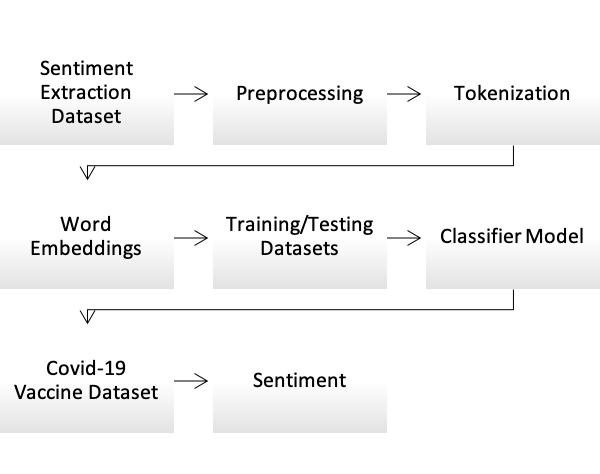
\includegraphics[width=0.45\textwidth]{NLPpipeline.png}
\caption{Flow diagram of NLP pipeline}
\label{fig:fig1}
\end{figure} 


\section{Results \& Analysis} \label{sec:results}
\subsection{Baseline Models}

\textbf{Single Layer LSTM}

Long Short Term Memory Recurrent Neural Network (LSTM RNN) in Figure \ref{fig:fig14} is tailored to learning sequence data \cite{huang2015bidirectional}. The model in this paper has a single LSTM hidden layer to extract features from the sequence and has an embedding layer as the input. This LSTM layer is followed by a Dense layer with a Dropout regularisation technique set to a fraction of 0.2 to interpret the LSTM output and improve model performance by reducing overfitting. Following the Dense layer is another Dense layer with three output and a 'Softmax' activation function so the output has the properties of a probability distribution. Since the model is learning a multiclass classification problem, therefore, a categorical crossentropy was used to calculate the loss function and 'Adam' optimization was implemented for the gradient descent. \\




\textbf{Bi-Directional LSTM}

A similar configuration to single layer LSTM was used but with bidirectional layers see Figure \ref{fig:fig12}. The bidirectional LSTM (BDLSTM) model had more trainable parameters and took longer to train. It involved duplicating the first recurrent layer in the network so that there were two layers side-by-side, then providing the input sequence as-is as input to the first layer and providing a reversed copy of the input sequence to the second \cite{zworld}.


\textbf{Single Layer CNN}
CNNs are generally associated with image recognition tasks. Such applications require two dimensional CNNs called Conv2D whereas tasks like feature learning of text require one dimensional CNN called Conv1D. In contrast to RNNs, they also require less time to train. The 1D CNN architecture in Figure \ref{fig:fig13} uses an Embedding layer as input followed by a Conv1D layer, pooling layer and then a prediction output layer. 
In our analysis a filter size of 32 and kernel size of 6 was found to give best accuracy. The kernel size in convolutional layer defines the number of words to consider as the convolution is passed across the input text. 
On the other hand Dropout regularization did not have an effect in improving model performance. 



\begin{figure}[h]
\centering
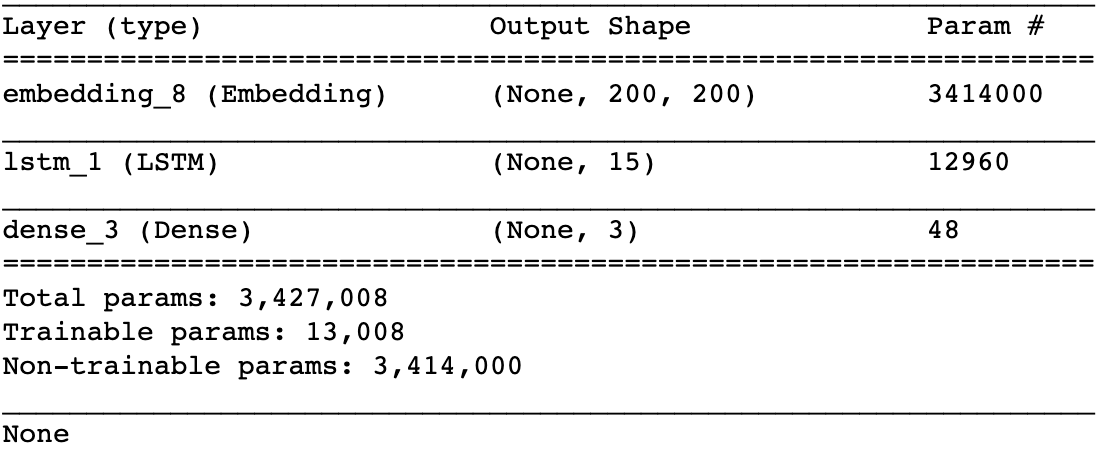
\includegraphics[width=0.45\textwidth]{singlelayerlstm.png}
\caption{Single Layer LSTM model summary}
\label{fig:fig14}
\end{figure} 

\begin{figure}[h]
\centering
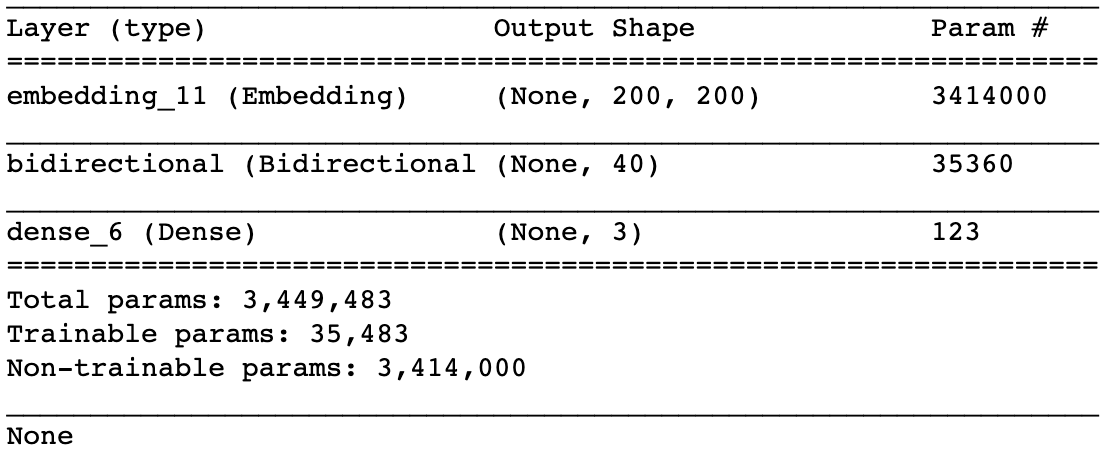
\includegraphics[width=0.45\textwidth]{bi-directional lstm.png}
\caption{Bidirectional LSTM model summary}
\label{fig:fig12}
\end{figure}  


\begin{figure}[h]
\centering
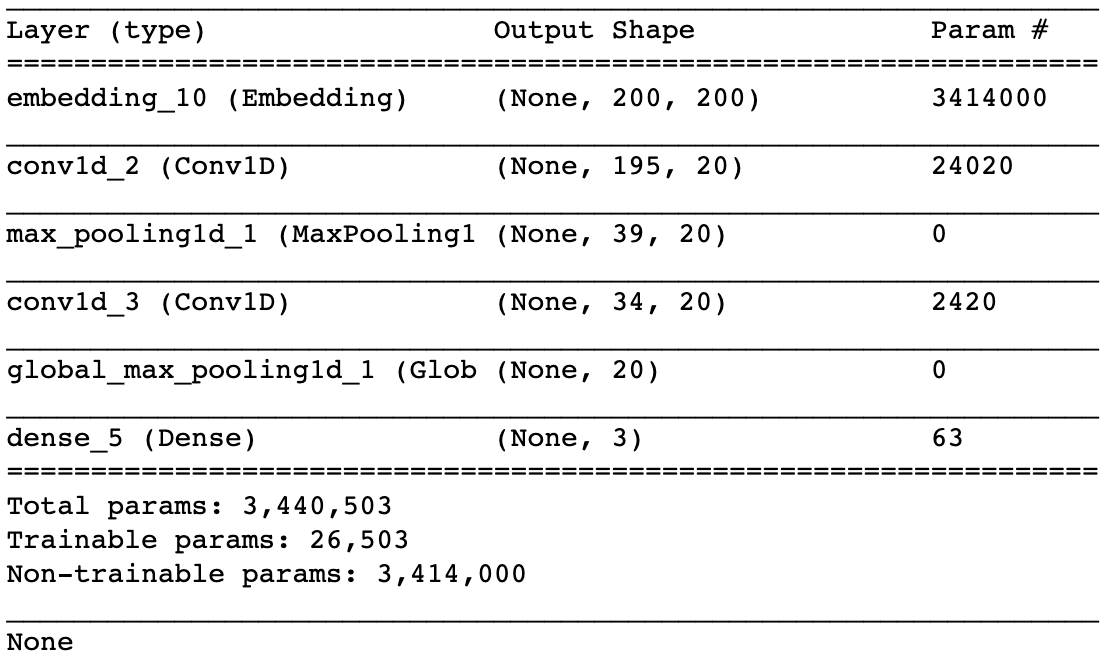
\includegraphics[width=0.45\textwidth]{1dcnn.png}
\caption{1D CNN model summary}
\label{fig:fig13}
\end{figure} 


\subsection{Multichannel Neural Networks}

Upon further investigation of the deep learning modelling techniques for sentiment analysis, we find that a deeper model with more layers for LSTM or CNNs deterred the model performance in contrast to the convention that more layers improve model's ability to learn features. As a result we opted for multichannel neural network architecture. The multichannel models consisted of two channels where the output of the two channel was concatenated into a single vector and processed by a Dense layer and an output layer (See Figure \ref{fig:fig28} - \ref{fig:fig32} in Appendix). The individual channels represent the baseline model configurations. By combining the three different baseline models we obtained the five different multichannel models. This allows the text to be processed at different resolutions (kernel size in CNN) or different embedding layers at a time, whilst the model learns how to best integrate these interpretations.  


\subsection{Comparison of Results}


\begin{table}[h!]
\centering
\caption{Comparison of performance of classifier models using confusion matrix}

\begin{tabular}{||c c c c||} 
 \hline
 Model & Positive & Neutral & Negative \\ [0.5ex] 
 \hline\hline
  LSTM & 0.45 & 0.96 & 0.28 \\
 BDLSTM & 0.47 & 0.96 & 0.31 \\ 
 CNN & 0.46 & 0.91 & 0.42 \\
 CNN+CNN & 0.52 & 0.95 & 0.31 \\
 LSTM+LSTM & 0.50 & 0.94 & 0.34 \\
 BDLSTM+BDLSTM & 0.48 & 0.97 & 0.22 \\
 LSTM+CNN & 0.47 & 0.95 & 0.35 \\
 BDLSTM+CNN & 0.49 & 0.94 & 0.36\\[1ex] 
 \hline
\end{tabular}

\label{table:2}
\end{table}

Before we can choose the model that performs the best for the task of sentiment classification on the Twitter Covid-19 Vaccine dataset, it is worth measuring how well it performs with its predictions. Looking at the confusion matrix we see how many negative tweets were classified as negative when they were actually negative and the same thing for positive and neutral tweets. The results of our confusion matrix of the baseline models and multichannel models are summarised in Table \ref{table:2}.  The model varies in results due to the stochastic nature of the algorithm but the average outcome is over 90\% for neutral, over 30\% for negative and over 45\% for positive tweets.\\

Due to the existing bias in the training dataset, where there were more neutral tweets, our classification model scored higher in neutral ratings. This means much of the negative and positive tweets are likely to get misclassified. For this reason we select a model that has a relatively higher negative rating as well as positive rating since most neutral ratings for all models are above 90\%. According to our selection method it is clear that single layer 1D CNN and Multichannel BDLSTM-CNN model stand out. We choose the simpler 1D CNN, because it results in shorter training time at 15s/epoch compared to 108s/epoch for the Multichannel Bidirectional-LSTM-CNN model.



\subsection{Classification of Covid-19 Vaccine Dataset}

\begin{figure}[h]
\centering
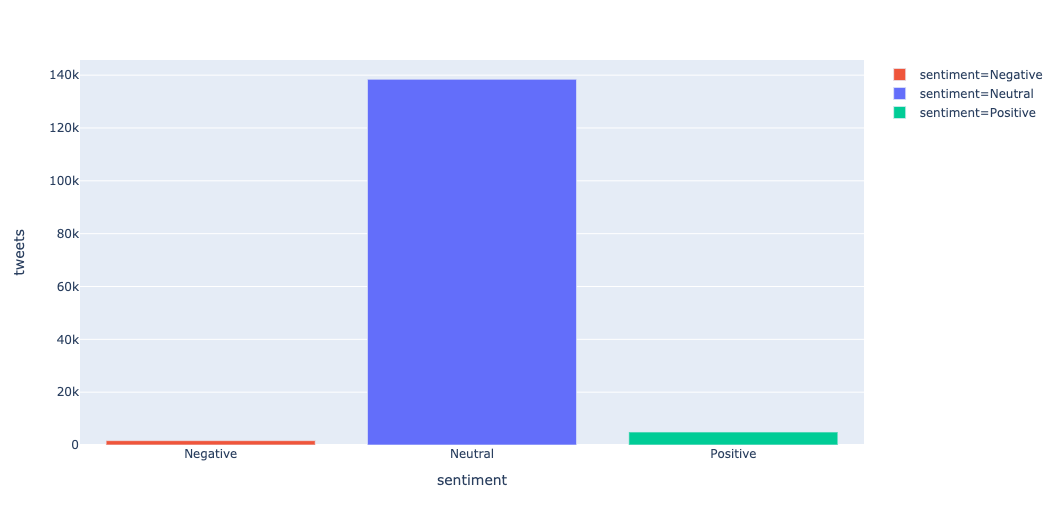
\includegraphics[width=0.45\textwidth]{newplot.png}
\caption{Resulting classification of tweets for each sentiment}
\label{fig:fig15}
\end{figure} 

Finally, at this stage the selected model-1D CNN-is repurposed for the classification of Twitter Covid-19 Vaccine dataset. The resulting sentiment analysis of the Transfer Learning method is displayed in Figure \ref{fig:fig15}. According to this classifier model there are 1,652 negative tweets, 138,847 neutral tweets and 4,926 positive tweets in the dataset. Upon inspection on the text classification of the tweets we extracted examples from the dataset in Figure \ref{fig:fig21} showing the three sentiment classes with instances of the associated tweet or phrase it has predicted the class for. However, there still exists misclassifications in the dataset due to the biases in the training dataset with more data skewed towards neutral class. 

\begin{figure}[h]
\centering
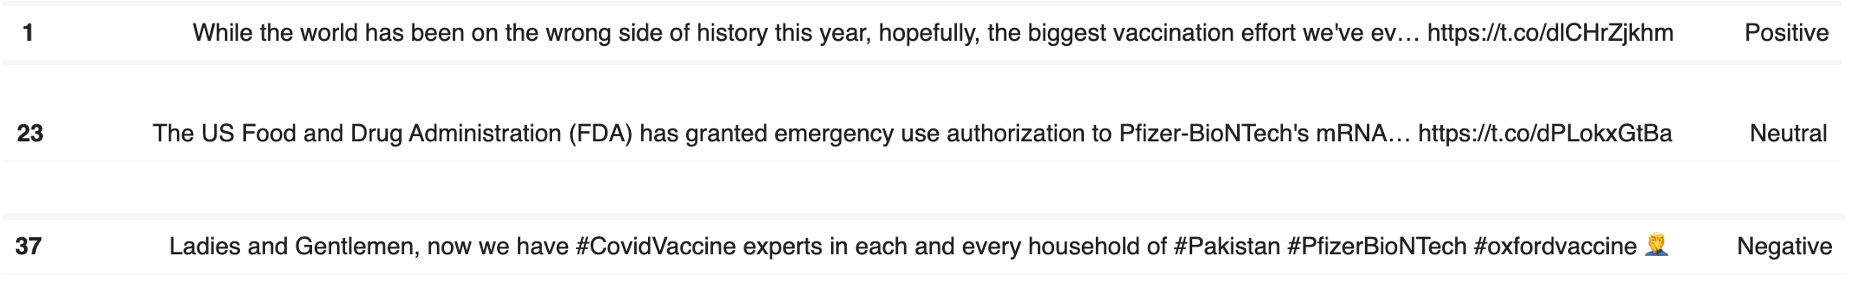
\includegraphics[width=0.45\textwidth]{classification.png}
\caption{Resulting classification of tweets for each sentiment}
\label{fig:fig21}
\end{figure} 


\subsection{Data Visualisation}

 \textbf{Time Series Analysis}
 
 \begin{figure}[h]
\centering
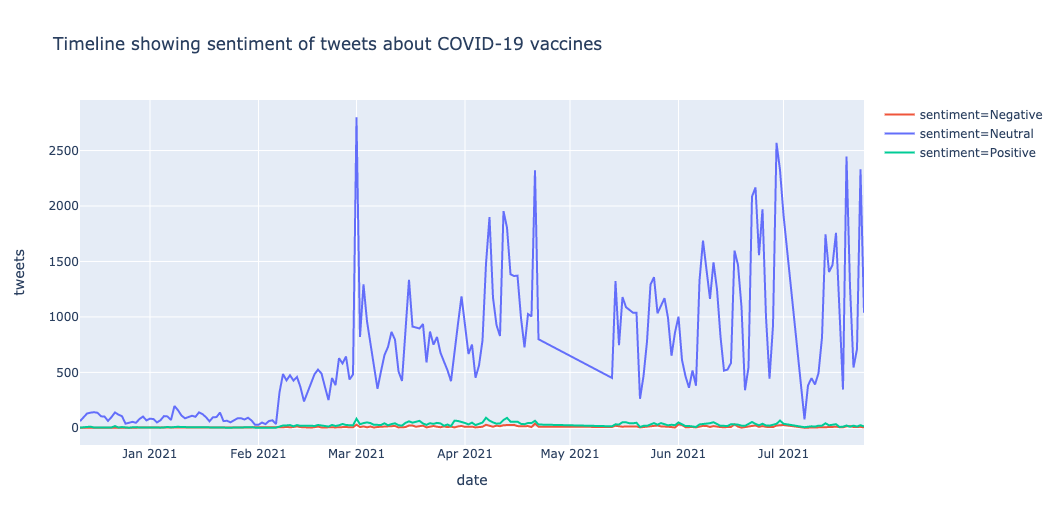
\includegraphics[width=0.45\textwidth]{vaccinetimeline.png}
\caption{Timeline of the distribution of the sentiments for all vaccines}
\label{fig:fig10}
\end{figure} 

\begin{figure}[h]
\centering
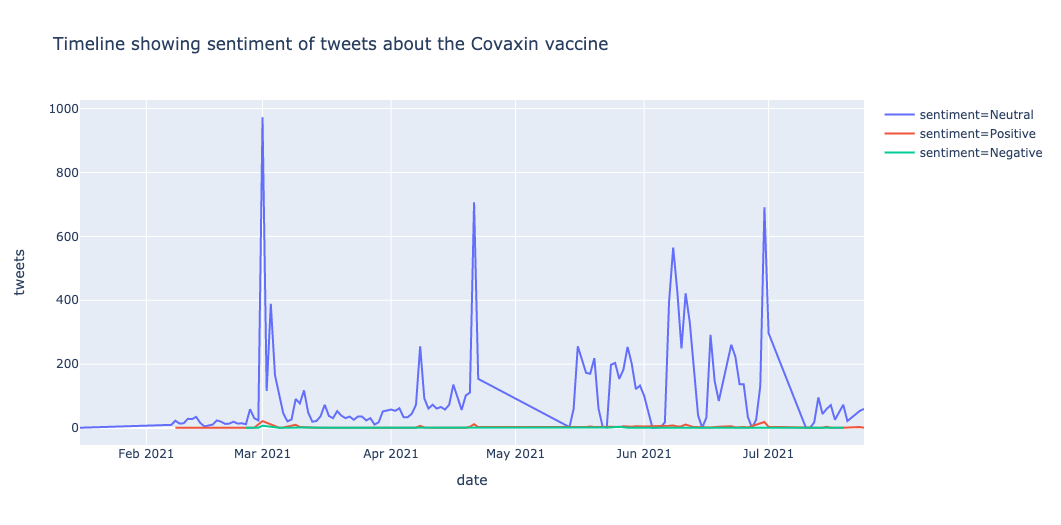
\includegraphics[width=0.45\textwidth]{covaxin.png}
\caption{Timeline of the distribution of the sentiments for the Covaxin vaccine.}
\label{fig:fig11}
\end{figure} 

\begin{figure}[h]
\centering
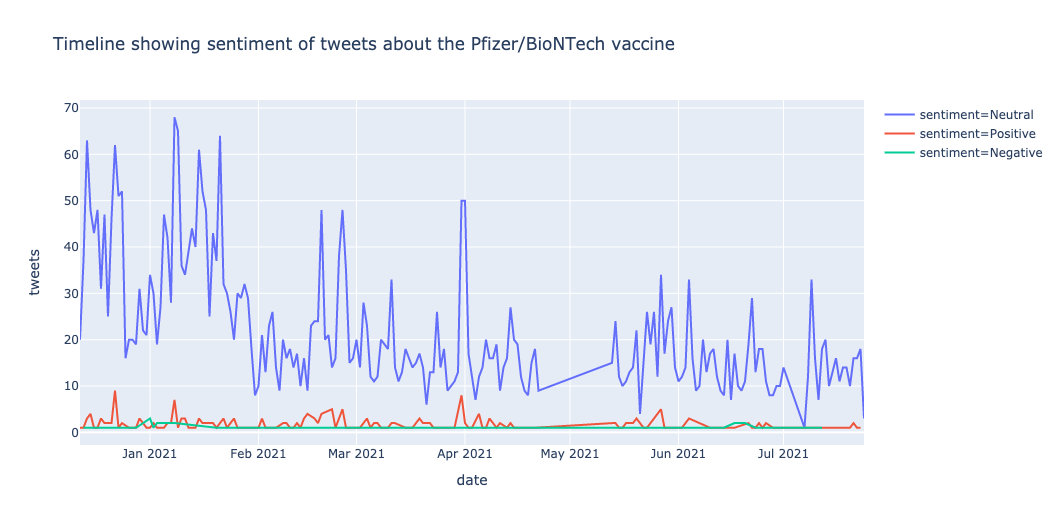
\includegraphics[width=0.45\textwidth]{pfizer.png}
\caption{Timeline of the distribution of the sentiments for the Pfizer/BioNtech vaccine.}
\label{fig:fig22}
\end{figure} 

Daily sentiments over the timeline series  were generated to identify the trend for the different Covid-19 vaccines in Figure \ref{fig:fig10}. The discussions around Covid-19 vaccines peak around March this was largely due to high ranking of the Covaxin vaccine related tweets from India, which can be seen in Figure \ref{fig:fig11}. We can use these graphs for further investigation of intriguing data using the direct reference to the timeline and corresponding sentiment spikes, for instance in Figure \ref{fig:fig22} we see that there has been a high rate of tweets consistently since the beginning of January 2021 relating to Pfizer/BioNtech Covid-19 vaccine. More graphs related to the other vaccines and their sentiments over a timeline is presented in Figure \ref{fig:fig23} - \ref{fig:fig27} in the Appendix.\\


 \textbf{Word Cloud Visualisation}
 
 
\begin{figure}[h]
\centering
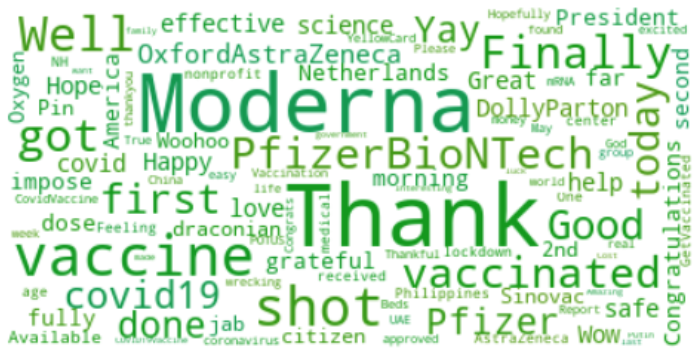
\includegraphics[width=0.35\textwidth]{positivecloud.png}
\caption{Wordcloud showing terms associated with positive sentiment around Covid-19 vaccine}
\label{fig:fig7}
\end{figure} 


\begin{figure}[h]
\centering
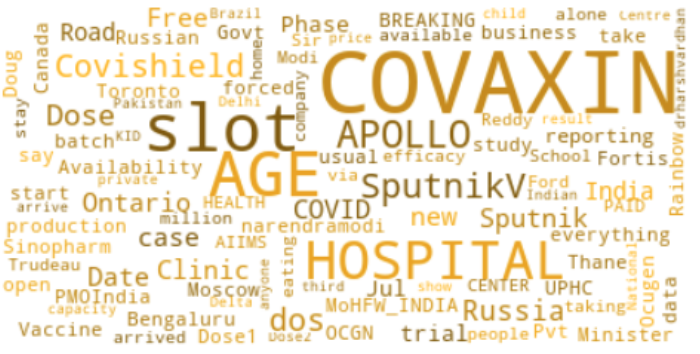
\includegraphics[width=0.35\textwidth]{neutralcloud.png}
\caption{Wordcloud showing terms associated with neutral sentiment around Covid-19 vaccine}
\label{fig:fig8}
\end{figure} 

\begin{figure}[h]
\centering
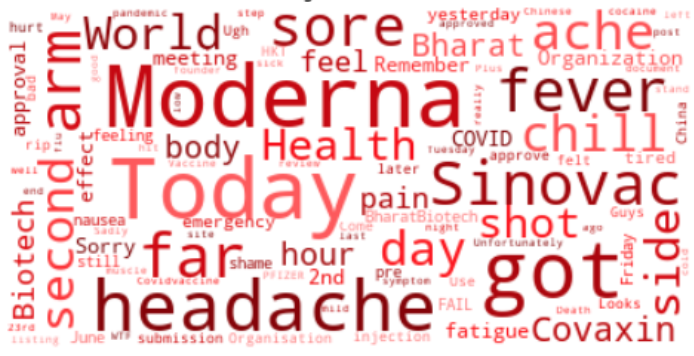
\includegraphics[width=0.35\textwidth]{negativecloud.png}
\caption{Wordcloud showing terms associated with negative sentiment around Covid-19 vaccine}
\label{fig:fig9}
\end{figure}  
 

In the final phase of the data analysis, color coded Word Cloud Visualisations were utilised to see which words were indicative of each sentiment. Such characteristic words can help tell a story through data visualisation.

Some of the characteristic words in the positive sentiment cloud in Figure~\ref{fig:fig7}  such as 'Shot', 'Safe', 'Vaccinated', 'Science', 'Moderna', 'Pfizer/BioNtech','Oxford astrazeneca', paints a picture of the frequented words since the start of the vaccine roll-out and generally expressing gratitude. This positive response appears to be from people who have received their first dose and those who got fully vaccinated. There is also positive reference to 'Dolly Parton' who helped fund Moderna's Covid-19 vaccine in the initial phase \cite{sworld}. There is also reference to UAE and China which were among the first countries to administer vaccines to the general public, also in recent times UAE has surpassed every other country in becoming most vaccinated country \cite{pworld}. 

Most of the neutral tweets in Figure \ref{fig:fig8} seem to be of informational nature with no emotional weight. It is noteworthy to mention that many of the negative tweets are likely to be classified as neutral due to inefficiencies in the classifier model. A closer inspection at the word cloud helps to make relations to everyday headline news for instance, it features words like 'Doug', 'Ford', 'Toronto', 'Trudeau', which upon investigation of the dataset sheds some light into the news of Canada's procurement of the covid-19 vaccine, which makes sense of its high ranking in the list of words. Upon further investigation we gain insight into the Indian-made Covaxin which is associated in the word cloud with the words - 'India', 'Modi', 'Covaxin' - referring back to the dataset the spike sheds light on the news headlines regarding the country's Prime Minister receiving the Covaxin vaccine dose around March 2021, which can also be connected back to the time series plots for Covaxin vaccine in Figure \ref{fig:fig11}.  

The negative tweets in Figure \ref{fig:fig9} seem to resemble the common reactions after receiving the second dose of the vaccines, these words included 'headache', 'fever', 'chill', 'sore', 'second', 'arm'. The negatively associated tweets around China's Sinovac vaccine is intriguing, upon further investigation it was found that the high frequency of the word was due to ongoing diplomatic issues. 


\section{Conclusions \& Future Work} \label{section:conclusion}
In NLP we see that a deeper more complex neural network does not necessarily mean a better neural netowork. We also see how a simple single layer 1D CNN allows us to classify an unlabelled twitter dataset for sentiment analysis of Covid-19 vaccines with the aid of Transfer Learning. Even though the resulting classifier model was not upto industrial standards in comparison to existing pre-trained models for NLP like VADER and TextBlob, it was still able to acheive a degree of success in automating the task of labelling tweetes based on the three sentiment classes. In addition to being repurposed for sentiment analysis the classifier model could be extended for different tasks such as topic modelling and spam filtering. In the future, this work will build upon the current neural network architecture by training the 1D CNN on a larger dataset which will directly improve the model's accuracy in classifying sentiments. More advanced capabilities will also be added to automate the task of sentiment analysis by using a webserver to host data visualisations with our model on live streaming tweets. \\


\section{Data Availability Statement}

The Twitter Sentiment Extraction dataset used in this paper is publicly available and downloadable from the following link ~\cite{bworld}

The Covid-19 All Vaccines Tweets - dataset used in this paper is also publicly available and downloadable from the following link ~\cite{cworld}


\bibliographystyle{unsrt}
\bibliography{IEEEexample}

\newpage

\section{Appendix}

\begin{figure}[h]
\centering
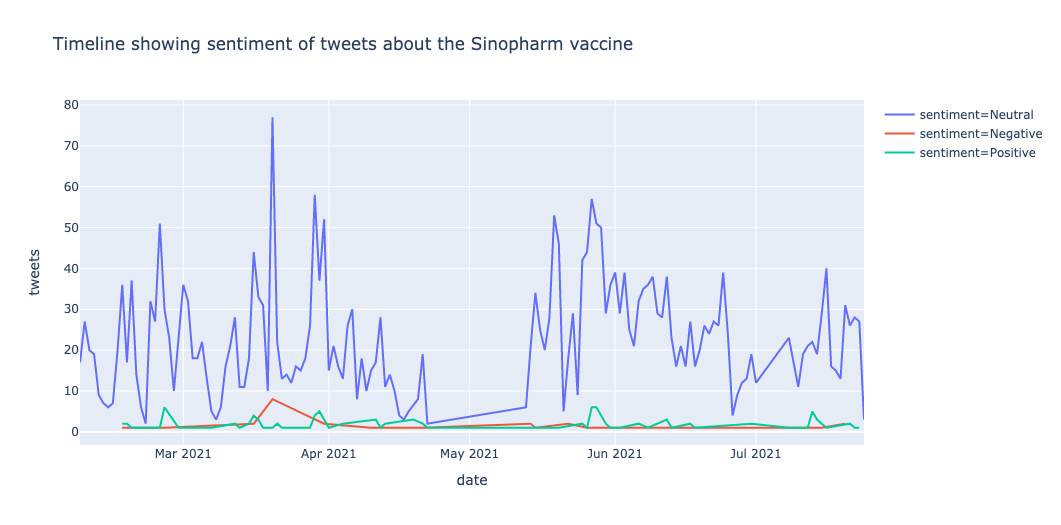
\includegraphics[width=0.35\textwidth]{sinopharm.png}
\caption{Timeline of the distribution of the sentiments for the Sinopharm vaccine.}
\label{fig:fig23}
\end{figure} 

\begin{figure}[h]
\centering
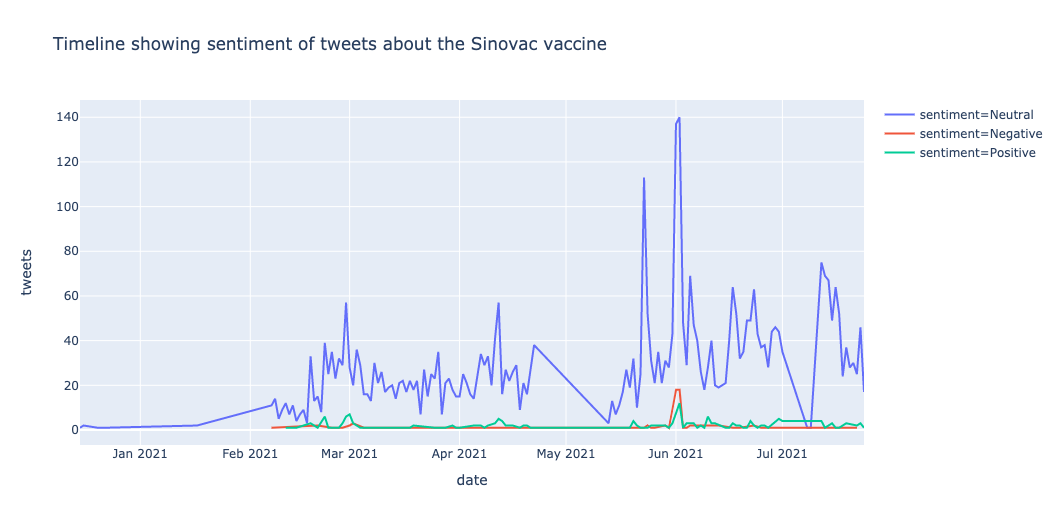
\includegraphics[width=0.35\textwidth]{sinovac.png}
\caption{Timeline of the distribution of the sentiments for the Sinovac vaccine.}
\label{fig:fig24}
\end{figure} 


\begin{figure}[h]
\centering
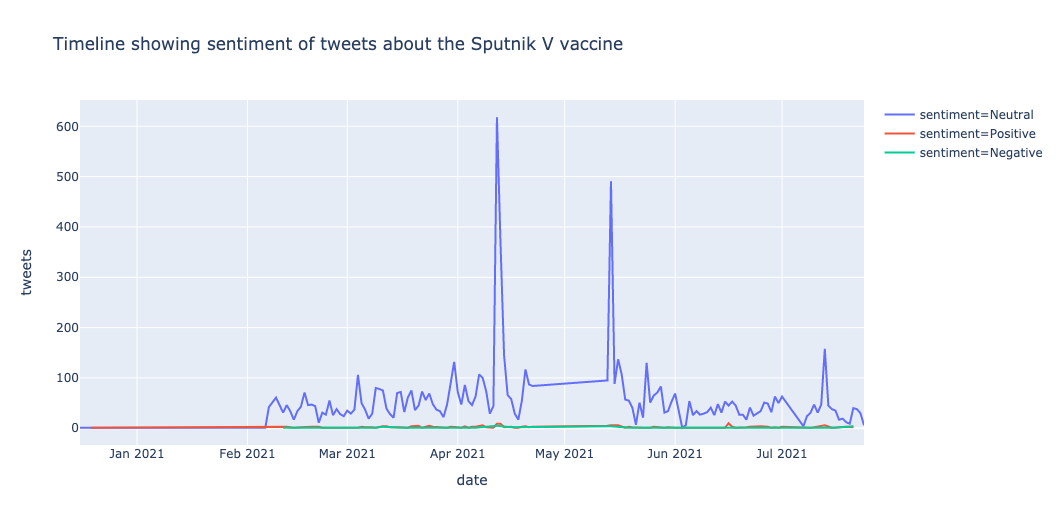
\includegraphics[width=0.35\textwidth]{sputnik.png}
\caption{Timeline of the distribution of the sentiments for the Sputnik V vaccine.}
\label{fig:fig25}
\end{figure} 


\begin{figure}[h]
\centering
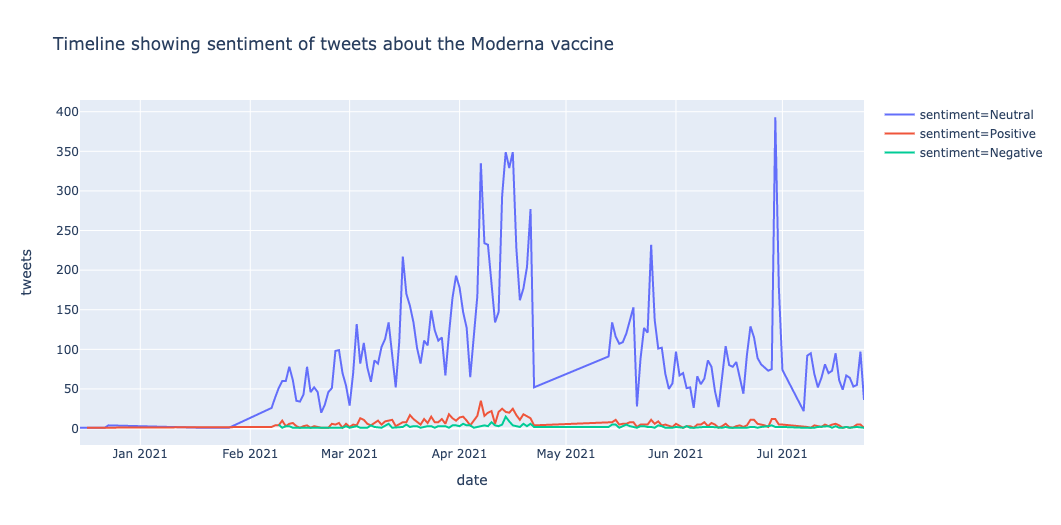
\includegraphics[width=0.35\textwidth]{moderna.png}
\caption{Timeline of the distribution of the sentiments for the Pfizer/BioNtech vaccine.}
\label{fig:fig26}
\end{figure} 

\newpage
\begin{figure}[h]
\centering
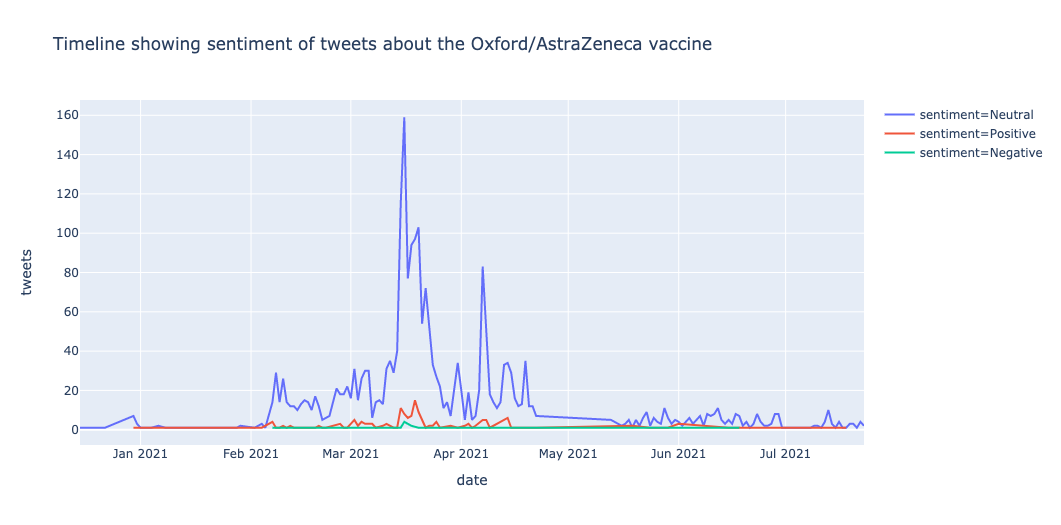
\includegraphics[width=0.35\textwidth]{oxford.png}
\caption{Timeline of the distribution of the sentiments for the Oxford/Astrazeneca vaccine.}
\label{fig:fig27}
\end{figure} 

\begin{figure}[h]
\centering
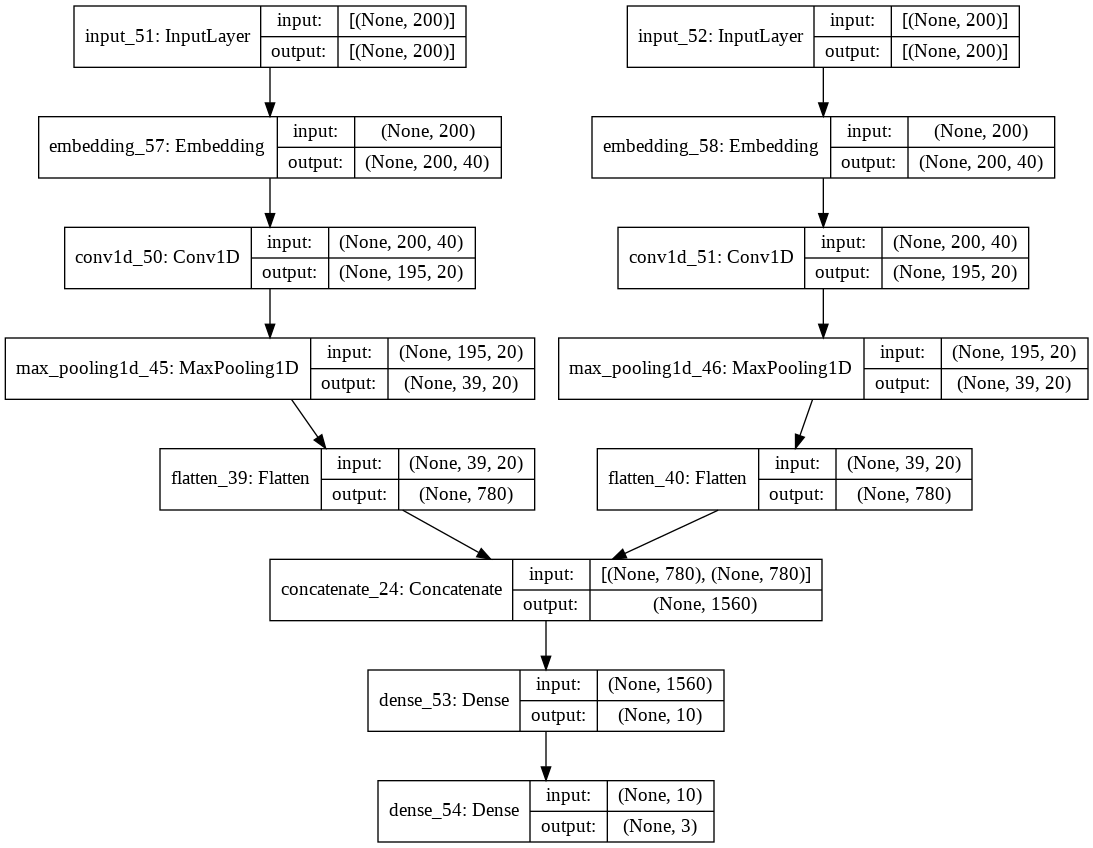
\includegraphics[width=0.35\textwidth]{multichannelcnn.png}
\caption{Model summary of Multichannel CNN}
\label{fig:fig28}
\end{figure} 

\begin{figure}[h]
\centering
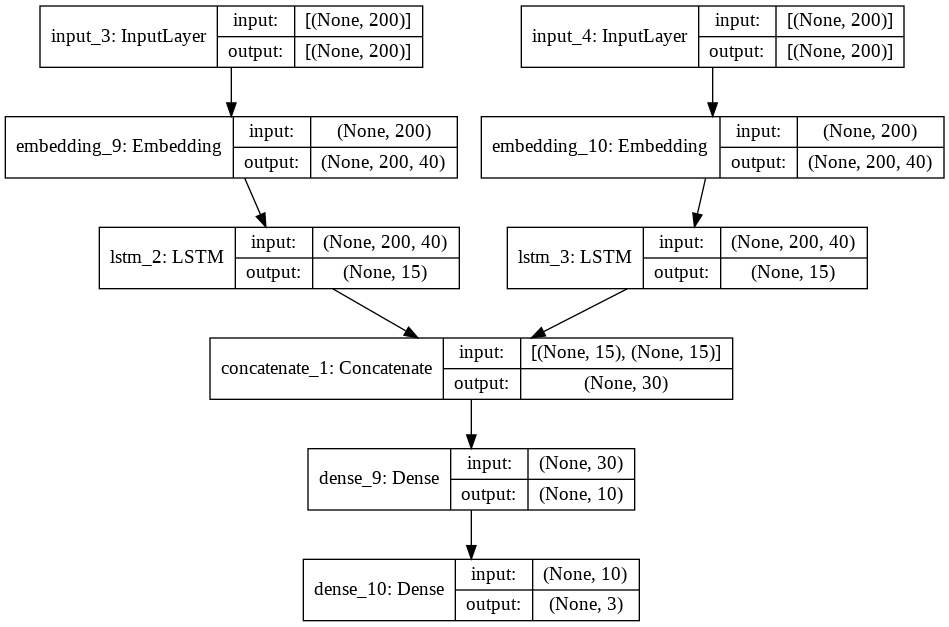
\includegraphics[width=0.35\textwidth]{multichannellstm.png}
\caption{Model summary of Multichannel LSTM}
\label{fig:fig29}
\end{figure} 

\begin{figure}[h]
\centering
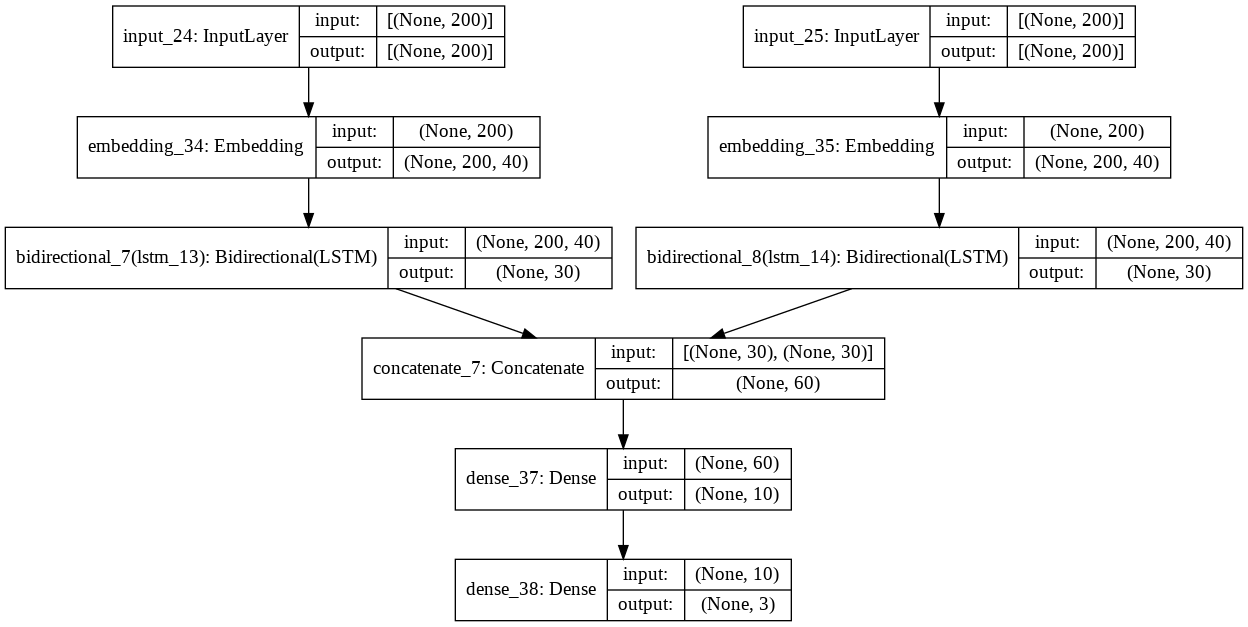
\includegraphics[width=0.35\textwidth]{multichannelbidlstm.png}
\caption{Model summary of Multichannel Bidirectional LSTM}
\label{fig:fig30}
\end{figure} 

\begin{figure}[h]
\centering
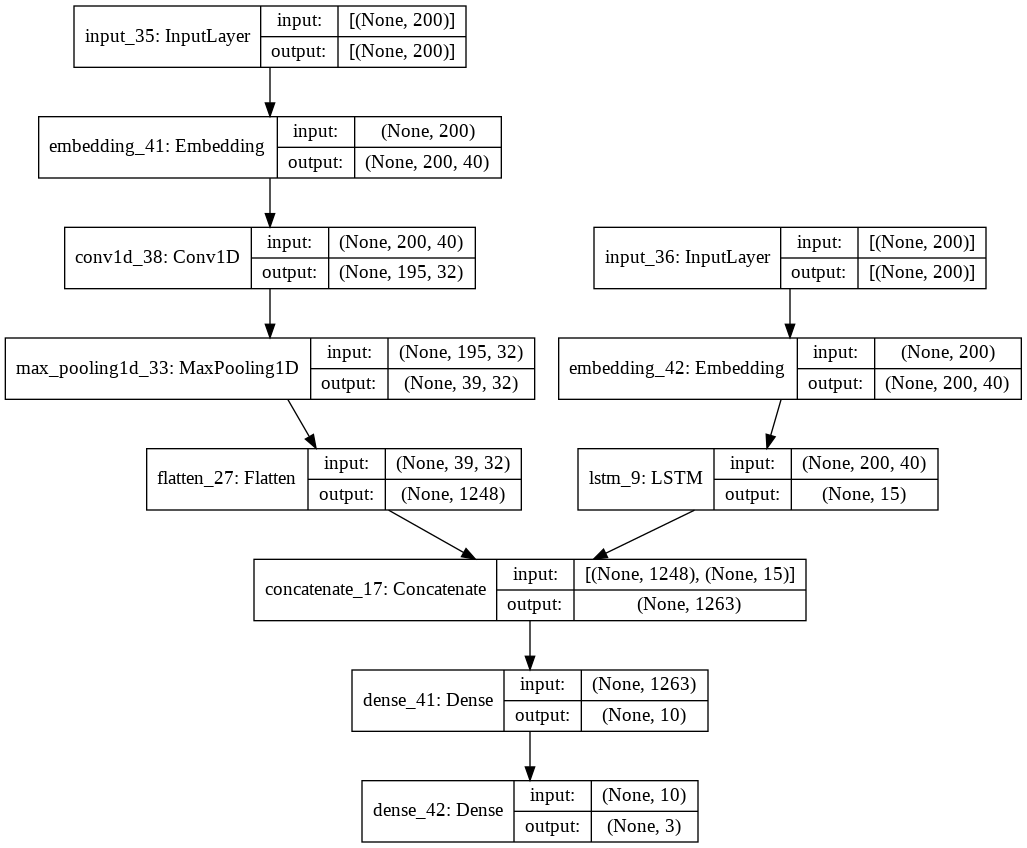
\includegraphics[width=0.35\textwidth]{lstm-cnn.png}
\caption{Model summary of Multichannel LSTM-CNN}
\label{fig:fig31}
\end{figure} 


\begin{figure}[h]
\centering
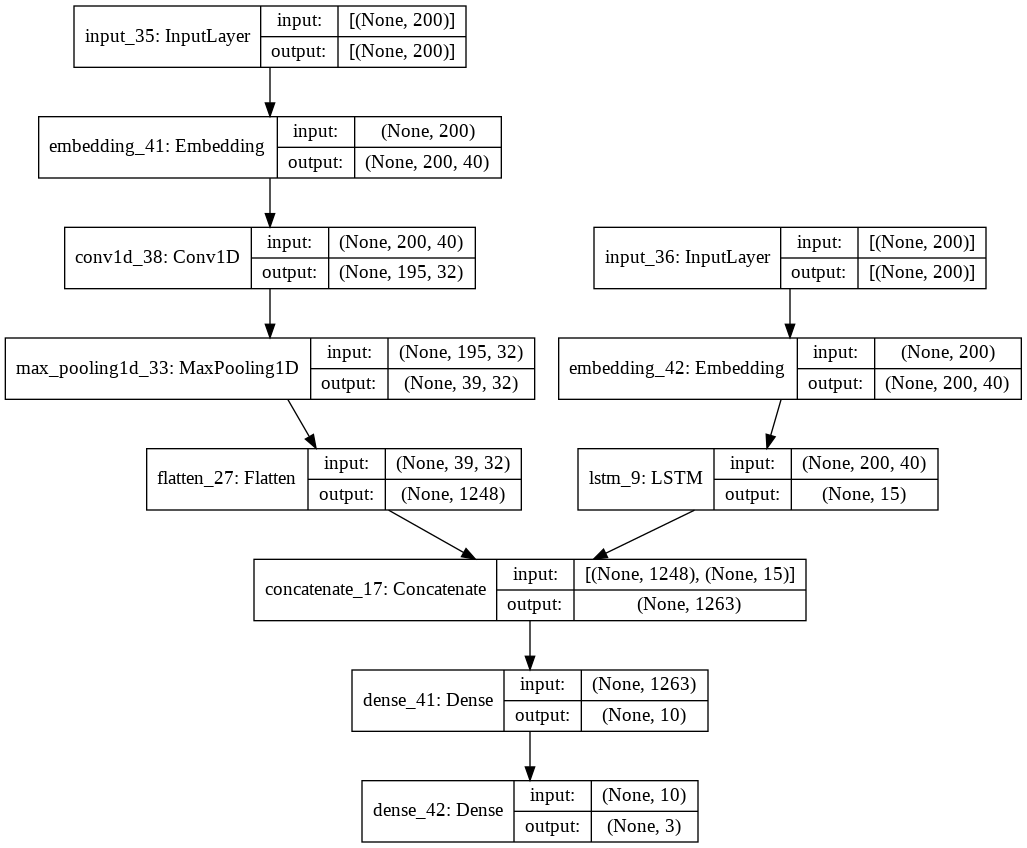
\includegraphics[width=0.35\textwidth]{bilstm-cnn.png}
\caption{Model summary of Multichannel Bidirectional LSTM-CNN}
\label{fig:fig32}
\end{figure} 

\end{document}
